\documentclass{standalone}
\usepackage{tikz}
\usepackage{ctex,siunitx,bm}
\setCJKmainfont{Noto Serif CJK SC}
\usepackage{tkz-euclide,ninecolors}
\usepackage{amsmath}
\usetikzlibrary{patterns, calc}
\usetikzlibrary {decorations.pathmorphing, decorations.pathreplacing, decorations.shapes}
\pgfdeclareverticalshading{pile}{100bp}{
  color(0bp)=(black);color(50bp)=(white);color(100bp)=(black)
}
\newcommand{\posthead}[2][gray]{
  \begin{scope}[#2]
    \fill[left color=#1,right color= #1,middle color=#1!20](0,0)ellipse(0.05 and 0.02);
    \fill[left color=#1,right color= #1,middle color=#1!20](0.05,0)rectangle(-0.05,0.07);
    \fill[left color=#1,right color= #1,middle color=#1!20](-0.06,0.07)arc(-180:0:0.06 and 0.02)--(0.06,0.15)--(0.05,0.16)--(-0.05,0.16)--(-0.06,0.15)--cycle;
    \fill[#1!50!gray](0,0.16)ellipse(0.05 and 0.02);
    \foreach \x in {75,45,15,-15,-45,-75}
    {
      \draw[very thin,#1!50!gray]({0.05*sin(\x)},{0.16-0.02*cos(\x)})--({0.06*sin(\x)},{0.15-0.02*cos(\x)})--++(0,-0.08);
    }
  \end{scope}
}
\begin{document}
\small
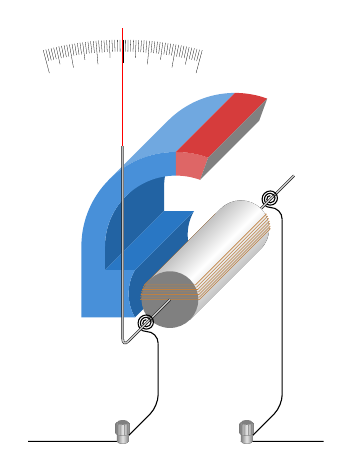
\begin{tikzpicture}[>=latex,scale=1.5]
  \begin{scope}[xshift=-0.25cm,yshift=-0.25cm]
    \fill[azure4](-0.6,0.2)--(-0.6,0.4)arc(180:135:0.6)--++(0.5,0.5)arc(135:180:0.6)--++(0,-0.2);
    \fill[azure4](150:0.4)arc(150:210:0.4)--++(0.5,0.5)arc(210:150:0.4);
    \fill[azure5](-0.1,0.7)--(-0.6,0.2)--(150:0.4)--++(0.5,0.5);
    \fill[azure7](0,1.2)--++(0.5,0.5)arc(90:135:0.8)--++(-0.5,-0.5)arc(135:90:0.8);
    \fill[azure6](150:0.4)arc(150:210:0.4)--(-0.8,-0.2)--(-0.8,0.4)arc(180:90:0.8)--++(0,-0.2)arc(90:180:0.6)--(-0.6,0.2);
    \fill[red6](0,1.2)arc(90:70:0.8)--++(-110:0.2)arc(70:90:0.6);
    \fill[red5](0,1.2)arc(90:70:0.8)--++(0.5,0.5)arc(70:90:0.8);
    \fill[gray]([shift=(70:0.6)]0,0.4)--++(70:0.2)--++(0.5,0.5)--++(-110:0.2);
  \end{scope}
  \begin{scope}[xshift=5.5mm,yshift=5.5mm]
    \draw[double=lightgray,line width=0.05mm](0,0)--(0.2,0.2);
    \draw[thin](0,0.03)arc(90:270:0.03)arc(-90:90:0.04)arc(90:270:0.05)arc(-90:90:0.06)arc(90:270:0.07)arc(90:0:0.1);
    \draw[double=lightgray,line width=0.05mm](0,0)--(-0.2,-0.2);
  \end{scope}
  \foreach \x in {0,5,...,30}
  {
    \draw[very thin,brown]([shift=(180-\x:0.25)]-0.3,-0.3)--++(0.6,0.6)--([shift=(\x:0.25)]0.3,0.3);
  }
  \fill[shading=pile,shading angle=45]([shift=(135:0.24)]-0.3,-0.3)--++(0.6,0.6)arc(135:-45:0.24)--++(-0.6,-0.6)--cycle;
  \fill[gray](-0.3,-0.3)circle(0.24);
  \foreach \x in {0,5,...,30}
  {
    \draw[very thin,brown]([shift=(\x:0.25)]0.3,0.3)--++(-0.6,-0.6)--([shift=(180-\x:0.25)]-0.3,-0.3);
  }
  \begin{scope}[xshift=-5mm,yshift=-5mm]
    \draw[double=lightgray,line width=0.05mm](0,0)--(0.2,0.2);
    \draw[thin](0,0.03)arc(90:270:0.03)arc(-90:90:0.04)arc(90:270:0.05)arc(-90:90:0.06)arc(90:270:0.07)arc(90:0:0.1);
    \draw[double=lightgray,line width=0.05mm,rounded corners=1mm](0,0)--(-0.2,-0.2)--(-0.2,1.5);
    \foreach \x in {105,100,95,90,85,80}
    {
      \draw[ultra thin] ([shift=(\x:2.6)]-0.2,-0.2)--++(\x:-0.2);
      \draw[ultra thin] ([shift=(\x-2.5:2.6)]-0.2,-0.2)--++(\x-2.5:-0.15);
      \foreach \y in {1,2,3,4,6,7,8,9}
      {
        \draw[ultra thin]([shift=(\x-0.5*\y:2.6)]-0.2,-0.2)--++(\x-0.5*\y:-0.1);
      }
    }
    \draw[ultra thin] ([shift=(75:2.6)]-0.2,-0.2)--++(75:-0.2);
    \draw[red,very thin](-0.2,1.5)--(-0.2,2.5);
  \end{scope}
  \draw[rounded corners](0.65,0.38)--(0.65,-1.2)--++(-0.3,-0.3)(-0.4,-0.67)--(-0.4,-1.2)--++(-0.3,-0.3)(0.35,-1.5)--(1.0,-1.5)(-0.7,-1.5)--(-1.5,-1.5);
  \posthead{xshift=0.35cm,yshift=-1.5cm}
  \posthead{xshift=-0.7cm,yshift=-1.5cm}
\end{tikzpicture}
\end{document}